\newpage
\chapter{Neuronale Netze}
Tauchen Sie ein, in die wundersame Welt der k"unstlichen Intelligenz. \\
Ich beschreibe hier einen neuralen Netzwerk Simulator, der auch von nicht-technischen Leuten,
einfach zu verstehen ist.
Basierend auf backpropagation'es Lernen f"ur das hier vorgestellte Tool, ist es m"oglich,
Ihren Computer zu trainieren und zu lernen, was Sie von ihm erwarten. \\
Ich m"ochte Ihnen zugleich einen Vorrausblick geben, was uns in naher Zukunft erwartet. \\

\section{Arten von Netzwerken}
Folgende neurale Netzwerke, werde ich hier noch vorstellen:\\
* ein Netzwerk, um die Zahlen 1, 2, und 3 zu erkennen. \\
* ein Netzwerk, um die logische Funktion AND zu verarbeiten. \\
* ein Netzwerk, um die logische Funktion XOE zu verarbeiten. \\

\section{Was sind Neuronale Netzwerke ?}
Expert Definition: \\
Ein neurales Netzwerk ist eine parallel-laufende Informationsstruktur.

\chapter{Sigmoid Funktion}
Eine Sigmoidfunktion, Schwanenhalsfunktion oder S-Funktion ist eine mathematische Funktion mit einem
S-förmigen Graphen.
Oft wird der Begriff Sigmoidfunktion auf den Spezialfall logistische Funktion bezogen,
die durch die Gleichung:\\
{\Large{$sig(t) = \frac{1}{1+e^{-t}} = \frac{e^t}{1 + e^t} = \frac{1}{2}*(1 + \tanh \frac{t}{2})$}}

\begin{figure}[h!]
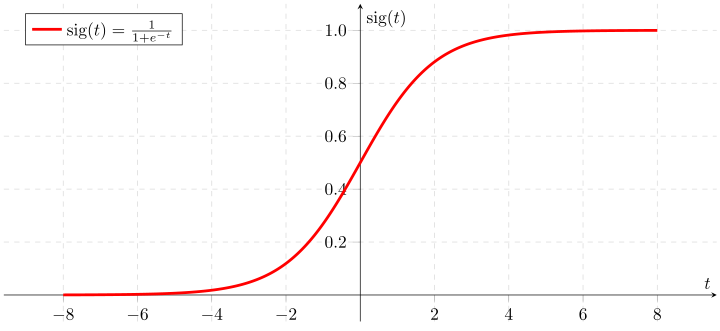
\includegraphics[width=0.7\linewidth]{pics/Sigmoid}
\caption{Graph der Sigmoid-Funktion}
\label{fig:Sigmoid}
\end{figure}
